\section{Related Works}

\begin{frame}{Explaining Counterexamples Using Causality}
    \begin{figure}
        \centering
        \frame{
            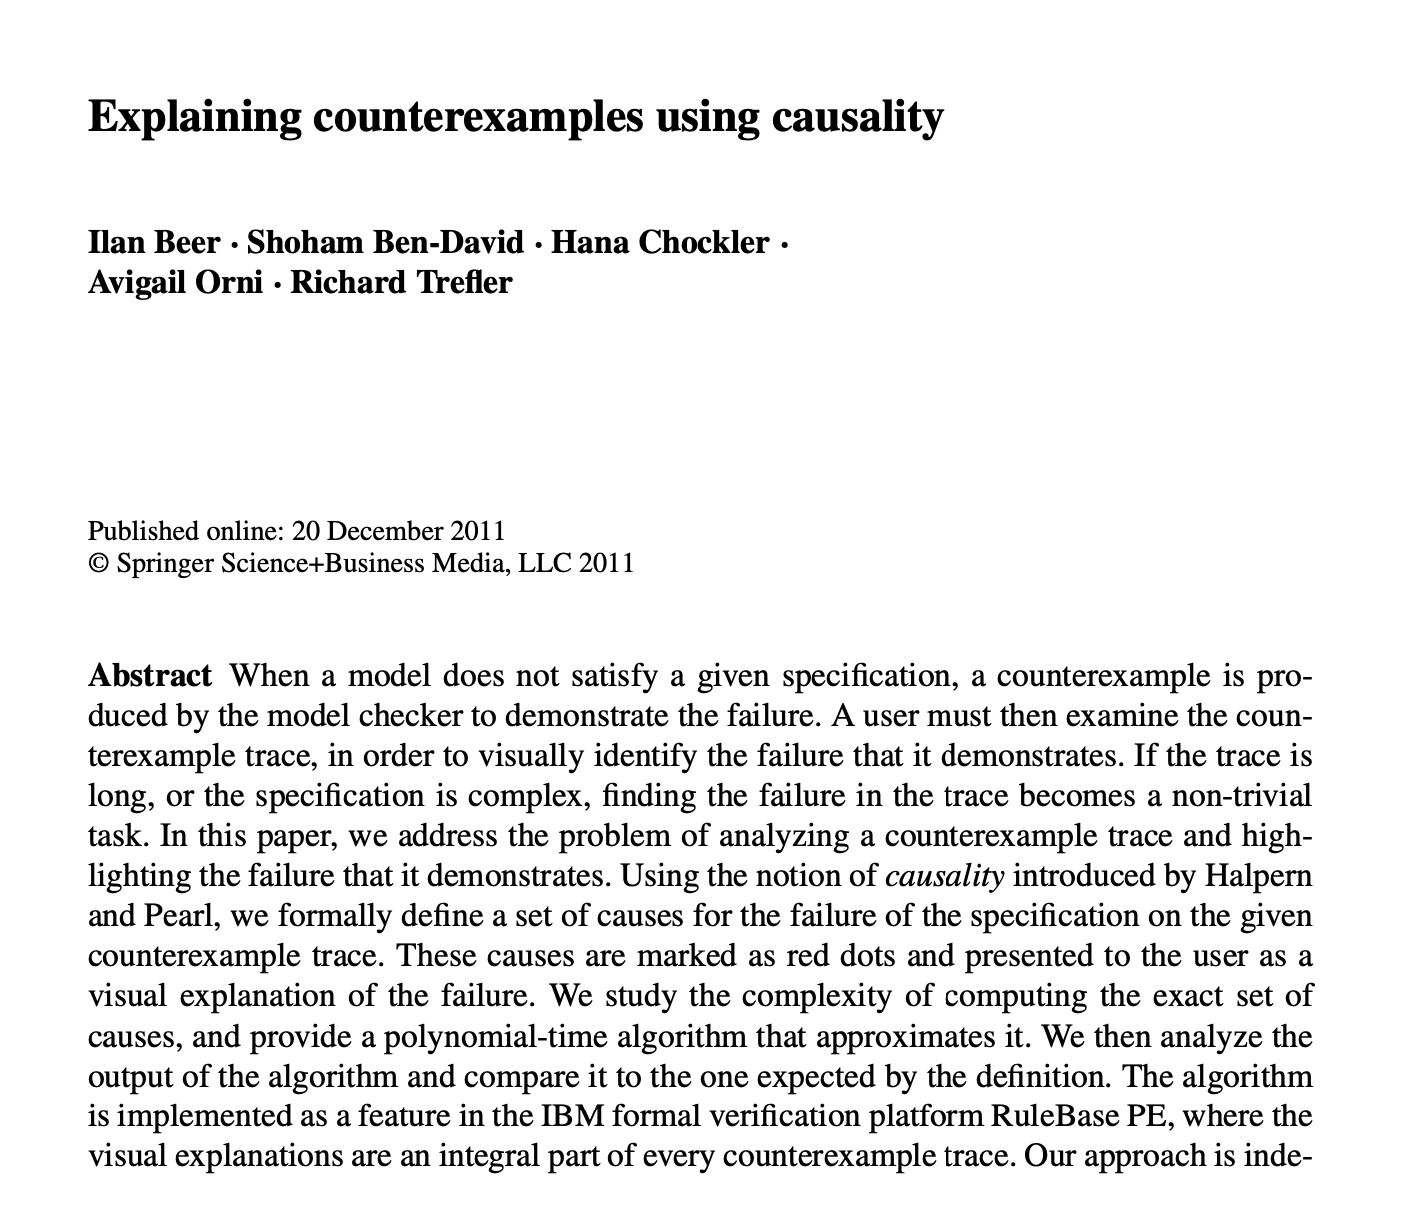
\includegraphics[width=8cm]{resources/chockler.png}
        }
    \end{figure}
\end{frame}

\begin{frame}{Explaining Counterexamples Using Causality}
    \begin{itemize}
        \item System is modelled with a Kripke structure
        \item The HP definition of actual cause is used to find the cause 
        of LTL property violation:
              \begin{equation*}
                  \boldsymbol{\mr{G}}((\neg \texttt{START} \wedge \neg \texttt{STATUS\_VALID} \wedge \texttt{END})
                  \ra [\neg \texttt{START}\ \boldsymbol{\mr{U}}\ \texttt{STATUS\_VALID}])
              \end{equation*}
        \item Pair of state and variables are considered as causes
    \end{itemize}
    \begin{figure}
        \centering
        \frame{
            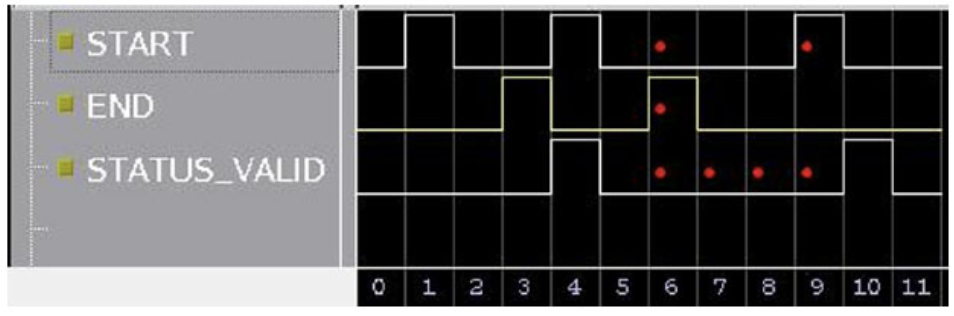
\includegraphics[width=8cm]{resources/chockler-ui.png}
        }
    \end{figure}
\end{frame}

\begin{frame}{Causal Reasoning for Safety in HML}
    \begin{figure}
        \centering
        \frame{
            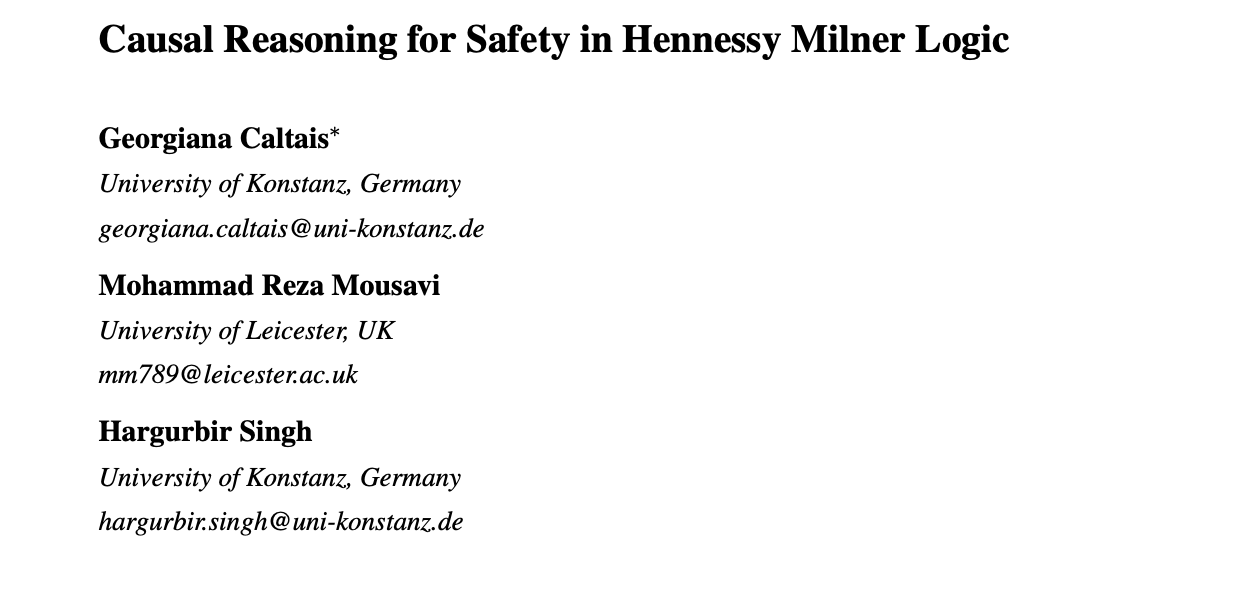
\includegraphics[width=8cm]{resources/hml-cause.png}
        }
    \end{figure}
\end{frame}

\begin{frame}{Causal Reasoning for Safety in HML}
    \begin{itemize}
        \item System is defined as a labeled transition system
        \item Properties are encoded in HML
        \item The HP definition is adopted for LTS and HML
        \item Example: causes for the property 
        $\his{h}\mathrm{T}$
    \end{itemize} 
    \begin{figure}
        \centering
        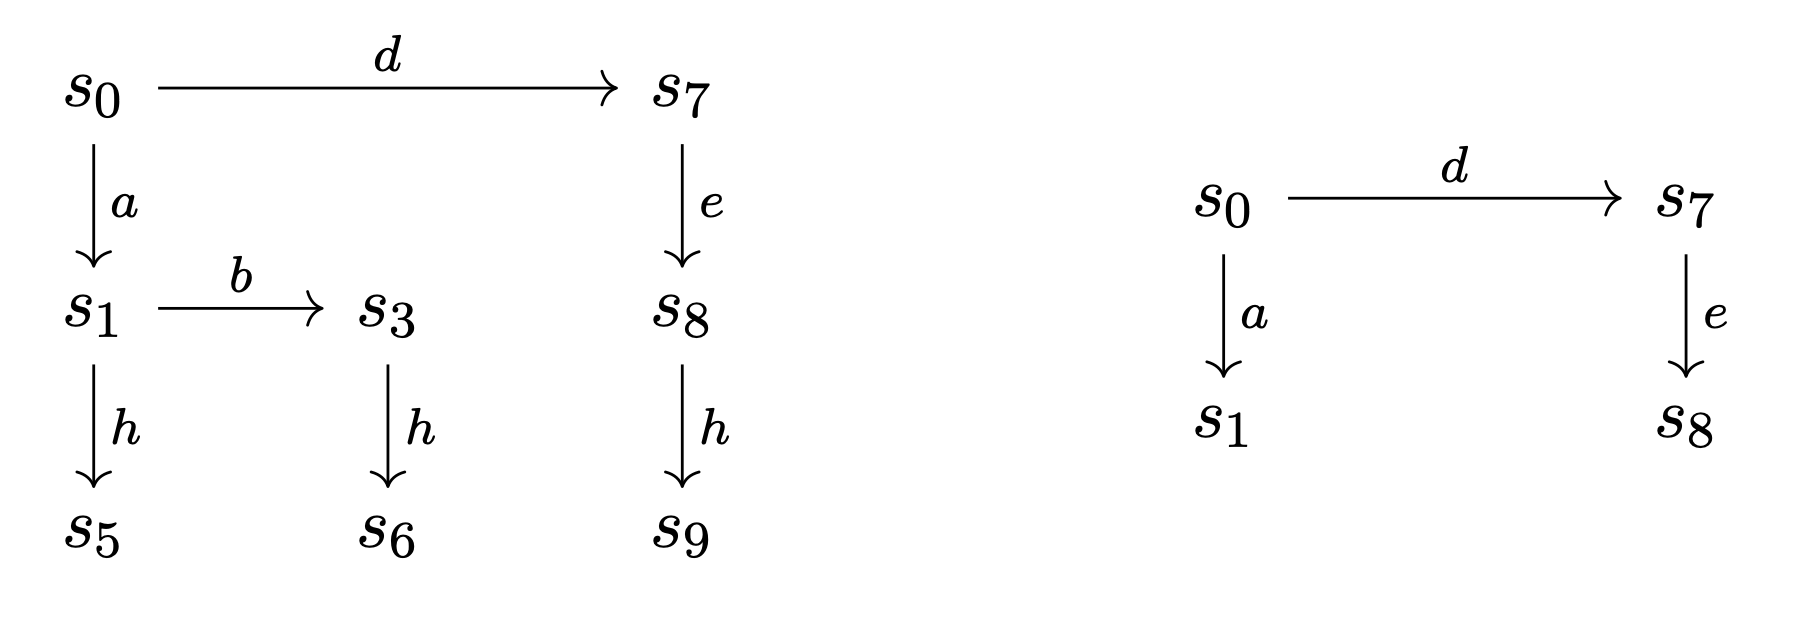
\includegraphics[width=10cm]{resources/hml-cause-example.png}
    \end{figure}
\end{frame}

\section{Conclusion}

\begin{frame}{Conclusion}
    \begin{itemize}
        \item Considering program constructs as causes
        \item Using a non-interleaving semantic 
        \item Direct usage of the actual cause definition
    \end{itemize}

    \vspace{\baselineskip}
    Future Works:
    \begin{itemize}
        \item Decomposing cause regarding the process constructs
        \item Purpose efficient (approximation) algorithm for finding 
        all causes
        \item Use the responsibility notion to compare and 
        rank the causes
    \end{itemize}
\end{frame}

\begin{frame}
    \begin{center}
        \Huge{Thank You!}
    \end{center}
\end{frame}